\documentclass{standalone}
\usepackage{tikz}

\usepackage{color}

\usetikzlibrary{arrows.meta}
\usetikzlibrary{calc}
\usetikzlibrary{shapes}
\usetikzlibrary{bending}
\usetikzlibrary{patterns}

\usepackage{gensymb}

\usepackage{pgfplots}
\usepackage{amsmath}

\DeclareMathOperator{\J}{J}

\begin{document}
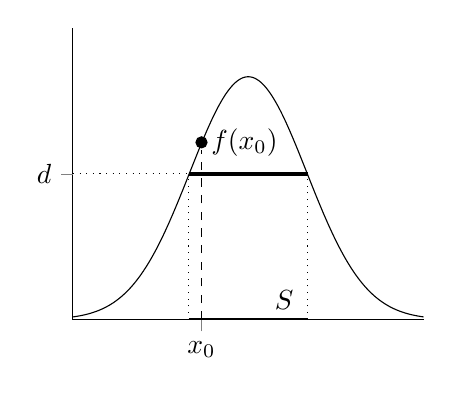
\begin{tikzpicture}[
	% scale=0.4,
	declare function={
		j(\x) =  exp(-\x*\x/50);	
	}
	]	
	
	\begin{axis}[
	axis on top=true,
	yshift=-4cm,
	scale=0.65,
	axis x line*=middle ,  axis y line*=left,
	xtick=\empty,
	ytick=\empty,
	extra y ticks = {0.6},
	extra y tick labels = {$d$},
	ytick align = outside,
	xtick align = outside,
	%xlabel = $x$,
	extra x ticks = {-4},
	extra x tick labels = {$x_0$},
	xlabel near ticks,
	ymin=0, ymax=1.2,
	xmin=-15, xmax=15]
	
	\addplot[domain=-15:15,samples=300]{j(x)};
	\addplot [black, mark = *, nodes near coords=$f(x_0)$,every node near coord/.style={anchor=180}] coordinates {( -4, 0.73)};
	
	\addplot[dotted, domain=-15:0]{0.6};

	\addplot[domain=-5.1:5.1, very thick]{0.6};
	
	\addplot[dashed]  coordinates {(-4,0) (-4,0.7)};

	\addplot[dotted]  coordinates {(-5.1,0) (-5.1,0.6)};
	\addplot[dotted]  coordinates {(5.05,0) (5.05,0.6)};
	\addplot[domain=-5.1:5.1, very thick]{0} node[pos=0.8] (S) {};
	\node [above] at (S) {$S$};
	
	%\addplot[domain=-1.3:2.9, very thick]{0};				
	
	
	\end{axis}
	
	
	\end{tikzpicture}  
\end{document}